\section{Internet-scale analysis}
\label{sec:internet-scale}

We explore how effective \name attacks might be in
practice by modeling the activity of Tor users, emulating the
corresponding Tor path selection of these users, and inferring  the
prevalence of AS-level adversaries who have the ability to
mount the attacks that we described in the preceding sections.

\subsection{Approach}

Figure~\ref{fig:simulations} summarizes our approach, which we detail in
the next section. We model the activity of Tor users and simulate
corresponding Tor path selection using TorPS~\cite{TorPS}.  TorPS
returns guard and exit relays, which we then feed as input---together
with source ASes and destination addresses---into our framework that
runs traceroutes from RIPE Atlas nodes.  The rest of this section
describes our approach in detail.

\subsubsection{Attack model}

\begin{figure}[t]
	\centering
	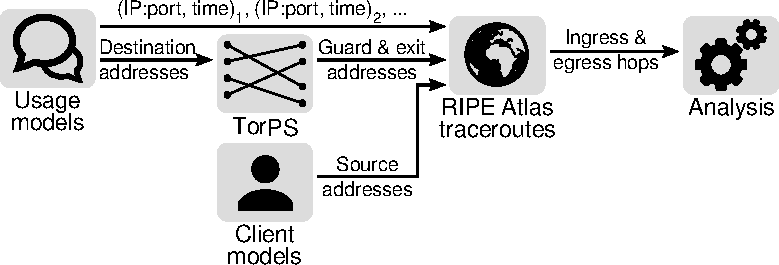
\includegraphics[width=\linewidth]{figures/simulations.pdf}
	\caption{The relation among our simulation components.  Our goal is to
	determine the ASes a Tor user's traffic traverses into and out of the Tor
	network.  Duplicate ASes on both sides can deanonymize streams.}
	\label{fig:simulations}
\end{figure}

We assume that an AS that can see traffic entering the Tor network and
and can see DNS traffic exiting the Tor network at the other end can use
this information in order to deanonymize the entering traffic.  Here we
seek to measure the chances an AS will be in this favorable position to
carry out such an attack.

A Tor exit can perform DNS resolution in two ways: running a name server
locally; relying on a third-party name server, such as its ISP's name
server or a public DNS name server such as Google's open public DNS
resolver ({\tt 8.8.8.8}).  In the case of Tor
exits that perform local DNS resolution a good position for an attacker
might be both (1)~anywhere on the AS path between a Tor client and a Tor
guard; and (2)~anywhere on the path between a Tor exit and any of the
name servers the exit has to communicate with to resolve the name.
These name servers include the root name server, the TLD servers, and
the second-level servers.  The ASes along the path from the exit relay
to the name servers will be able to see the domain names that the exit
relay is querying.

For Tor exits that rely on a third-party for DNS resolution, an
adversary might be on the path between a Tor client and a
Tor guard and on the path between a Tor exit and the third-party name
server.  \fixme{QUESTION: ``In addition, the DNS queries will look like they are coming
from the IP address of the name server and not the IP address of the
exit relay.''--This new wording seems unclear to me now--wanted to say 
that ASes on the path from the 3rd-party to the DNS servers will see that 
the queries are coming from the 3rd-party and not the exit IP, which is 
why we ignore them . . .}

\subsubsection{Simulating Tor user activity with TorPS}

To measure the likelihood that an AS can be in a position to perform a
\name attack, we use TorPS, the Tor Path Simulator, which mimics how the
Tor client software constructs circuits.  TorPS thus provides realistic
combinations of guards and exits based on the state of the Tor network
at a given time. TorPS is based on Tor stable release version 0.2.4.23. 
For each sample, 
it uses one guard which expires after 270 days. We use TorPS to emulate
the behavior of a Tor client for the month of March 2016.  As in
previous work, we perform 100,000 samples in the TorPS Monte Carlo
simulation.  

For our simulation, we had each client visit several websites every day for
March 2016.  We modeled our client behavior off of the ``Typical'' model 
used in~\cite{Johnson2013a}.  At 9am we have the client visit Gmail and Twitter.  
At 12pm the client visits Google Calendar and Google Docs. At 3pm the client 
visits Facebook and Instagram. Finally, at 6pm and 6:20pm the client visits Google, 
Startpage, and Ixquick.  (Note: For our chosen websites and port (443), 
Torps provided a new circuit every 10 minutes.  It did not provide a new circuit 
for different websites if the client visited them within the same 10-minute windows. 
This is in contrast to how the latest Tor Browser works where it will provide a new 
circuit every time you visit a different website even if 10 minutes have not passed.  
Thus, our results will be conservative in this respect.)  Also, in our study each 
client sample had 372 opportunities to be compromised in March because there are 31 
days in March, and our client visits 12 sites per day.

Finally, we had to choose where to place our clients. That is, we had to choose 
which ASes we wanted our sample clients to be using Tor from.  We first found 
out what the most popular countries for Tor users were from~\cite{metrics-countries} 
and chose the top five.  
We then researched which ISPs seemed to be the biggest players in those markets, and 
used those AS numbers for our client ASes.  For the United States, we chose Comcast 
(AS 7922).  For Russia we chose Rostelecom (AS 42610).  For Germany we chose 
Deutsche Telekom (AS 3320).  For France we chose Orange (AS 3215).  And for Great 
Britain, we chose British Telecom (AS 2856).  

%Thus, each guard-exit pair had 744 opportunites to be
%compromised (this assumes that the circuit changes for every visit to
%{\tt domain.com}).
% It is much better to use a tool like TorPS in order to
%measure these chances instead of just using all permutations of guard and exits.

%The paragraph changes a lot: Made our own model based off of UGR ``typical'' model.  
%The sample user visits nine websites during the course of his day: mail.google.com, 
%twitter.com, calendar.google.com, instagram.com, startpage.com, ixquick.com, docs.google.com, 
%facebook.com, and google.com.  \fixme{Should we mention the fixes we made to TorPS? Should we mention 
%the problem we found with their user models? YES. -- I don't think it's relevant here anymore 
%because we're not doing the traditional (exit ip - website destiation) traceroutes, like they did.}




\subsubsection{Inferring AS-level paths: traceroute + {\tt pyasn}}


% - 197 out of all 377 (52%) Tor exit ASes have Atlas probes.
% - 220 out of all 434 (51%) Tor guard ASes have Atlas probes.

% - Atlas ASes cover 57.53% of Tor exit bandwidth.
% - Atlas ASes cover 73.59% of Tor guard bandwidth.

\begin{table}[t]
	\renewcommand{\tabcaptext}{The coverage of RIPE Atlas nodes that are colocated with Tor guard and exit
	relays.}
      \topcap{\tabcaptext}
	\centering
	\begin{tabular}{l|r r}
	\toprule
	\textbf{Atlas probe coverage} & \textbf{Tor guard ASes} & \textbf{Tor exit ASes} \\
	\midrule
	By bandwidth & 73.59\% & 57.53\% \\
	By number & 50.69\% & 52.25\% \\
	\bottomrule
	\end{tabular}
        \bottomcap{\tabcaptext}
	\label{tab:atlas-coverage}
\end{table}


The Internet-wide experiment requires inferring the AS-level paths from
each exit relay to each destination. We decided against the (more
commonly applied) AS path inference because Juen \ea showed that it can
be quite inaccurate~\cite{Juen2015a}.  Using traceroute can yield more
accurate paths.  Measuring traceroutes from client to guard notes is
straightforward: we simply select a probe in a client AS and perform
traceroutes to each respective guard. %Wow, nice story here! Thank you!

Measuring traceroutes from exit relay to destination is far more
difficult because Tor does not implement a mechanism to facilitate
traceroute~\cite{Murdoch2007a}.  One approach, used in previous
work~\cite{Juen2015a}, is to ask relay operators to perform traceroutes.
Unfortunately, this approach only yielded traceroutes from relays
representing 26\% of exit bandwidth.  Instead, we observe that RIPE
Atlas~\cite{atlas} has probes in many ASes that have Tor exit relays.
We used this insight to design a measurement experiment to run
traceroutes from RIPE Atlas probes that were located in the same ASes as
Tor exits, to each of the destinations in question.  As shown in
Table~\ref{tab:atlas-coverage}, for a day in May 2016, we found that
RIPE Atlas had probes in 52\% of ASes that contain Tor exit relays.  We
found that RIPE Atlas has probes in 51\% of ASes that contain Tor guard
relays.  More importantly, we found that Atlas ASes cover 58\% of Tor
exit \textit{bandwidth} and 74\% of Tor guard bandwidth. (This statistic
is important because Tor relay usage is not evenly split among all of
the relays.) We considered using PlanetLab to initiate traceroutes, but
unfortunately most PlanetLab nodes are located in research and education
networks~\cite{banerjee2004interdomain} and are thus not well-suited for
performing these types of measurements.

%The traceroutes are from July 2016, and we applied these in our analysis of Tor 
%in March 2016.  \xxx{don't understand what ``analysis of Tor in March
%  2016'' means.  What's the Tor trace corresponding to this?} \xxx{The following sentence should 
%explain it better, please, although now I'm thinking it doesn't matter as much as I thought it did 
%because we're working at the AS level.
%--The point is that although we're simulating the March 2016 Tor situation, the traceroutes themselves 
%are from July 2016 because I had to rerun all the traceroutes and add a bunch because we were no longer 
%using nymity nor 
%the original client AS. We upgraded the model and made the client visit 9 different websites from 5 
%different client ASes. We had to stick with March because we didn't have ``Status Quo'' information 
%from July. Summary: The results would perhaps be even more accurate if 
%all these brand new traceroutes had been 
%run closer to March 2016. Do we need to mention this??}


Moved the following out of the Results section--will come up with either a header and/or an 
opening sentence:
%In contrast to how TorPS is used in~\cite{Johnson2013a}, we do not ultimately run 
%traceroutes from .
Describe the four scenarios in the graph here: 1) ISPs, 2) Google, 3) Local, and 
4) Status Quo.

we only concern ourselves with root domain, that is, if facebook.com, we don't 
take the embedded URLs into account.

%Traditional: ``Traditional'' represents the paths between all exit ASes that RIPE Atlas 
%has coverage for and domain.com. That is, this measurement doesn't take DNS into account 
%at all, as has been traditionally done.

\begin{itemize}
    \item \emph{ISPs:} ``ISPs'' represents what would happen if all exit relays used their ISPs' DNS name 
servers.  We choose to represent this by saying that the name server is in the same AS as the 
exit relay.

    \item \emph{Google DNS:} ``Google DNS'' represents what would happen if all exit relays used 
Google's public DNS resolver ({\tt 8.8.8.8}) for resolution. We ran traceroutes from probes in all the exit 
ASes that RIPE Atlas had coverage for to  {\tt 8.8.8.8}.

    \item \emph{Local:} ``Local'' represents what would happen if all exit relays ran their own name 
servers locally (e.g., the use of unbound) on their own machines. In order to figure out 
what ASes would be traversed on the way to resolve domain.com. In order to figure out the 
DNS delegation path, we use the command line option \texttt{+trace} of the
command line tool dig. Assuming no caching and assuming 
iterative resolution, for domain.com the name server will have to visit three name servers:
a root name server, a top level domain name server, and a second-level domain name server. 

    \item \emph{Status Quo:} ``Status Quo'' represents to the best of our ability the 
type of name resolution 
that exit relays perform, whether that be their own or the use of 3rd-party name servers, 
which again includes public DNS name servers and their ISPs' name servers.  To figure this 
out, we used the exitmap tool, our own website, and our own authoritative name server 
in order to figure out the IP addresses of the name servers that the exit relays were 
using. We then performed traceroutes from the exit ASes to the appropriate IP addresses 
in order to get the AS-level paths.
\end{itemize}


Given these traceroutes, we mapped each IP address in every traceroute
to a corresponding AS.  The Python {\tt pyasn} module relies on BGP
routing tables to perform these mappings; by using a routing table that
coincides with the time when we performed our traceroutes, we can obtain
accurate AS-level mappings.  (This method of course is subject to
inaccuracies in the event of BGP route hijacks or leaks, but we expect
those events to be relatively unlikely for the time period and IP
prefixes that we are concerned with.)  (Please note that although we're 
analyzing Tor during the month of March 2016, we ended up using traceroutes from 
July 2016 due to information we didn't have time to collect again.  We recognize 
that it would have been better for our traceroutes to be closer in time to the 
month we wanted to analyze, but we don't 
believe that this should greatly affect our results, and spot checks confirm 
this.)  



% \fixme{Get the numbers from my data for the fan-out.}
\subsection{Results}

\begin{figure}[t]
\centering
\subfigure[Number of compromised streams.]{
	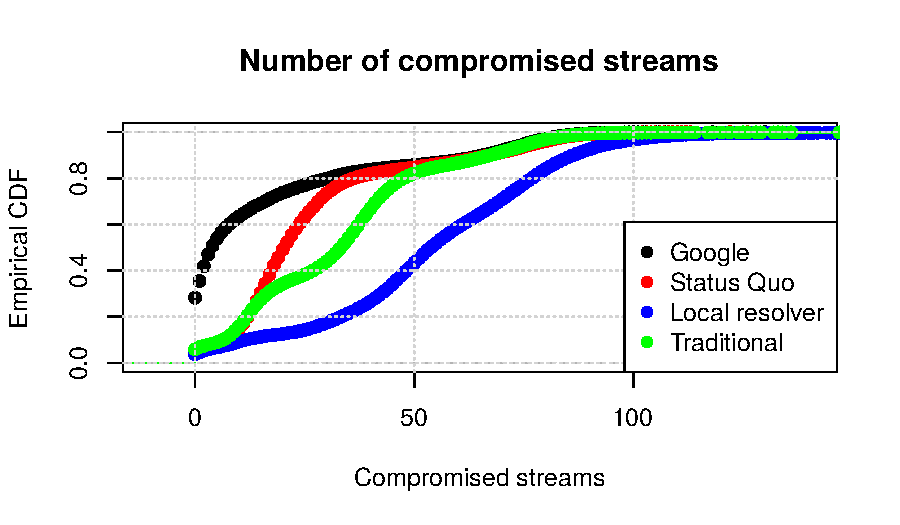
\includegraphics[width=0.465\linewidth]{figures/num-compromised-streams.pdf}
    \label{fig:compromised-streams}
}
\subfigure[Time to first compromise.]{
	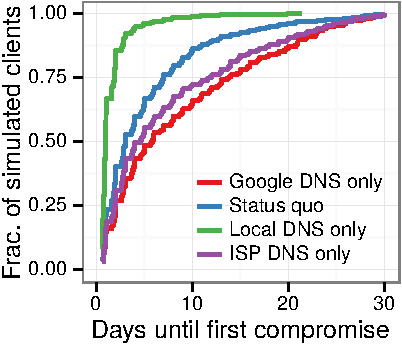
\includegraphics[width=0.465\linewidth]{figures/time-until-compromised.pdf}
    \label{fig:time-until-compromise}
}
\caption{Two emulations for the Tor network in March 2016 show the
  number of compromised streams and the time until the first compromised
  stream.} 
\label{fig:compromise-stream-time}
\end{figure}

Figures~\ref{fig:compromised-streams}
and~\ref{fig:time-until-compromise} show that
\fixme{will insert the 5 figures soon, the discrepancy with the ISPs' time-to-compromise
looking better than Google's will be fixed, too (figured out why that was happening)}
ISPs fared much better than the other situations. Google was next. There is a potential 
tradeoff between the safety of using a well-managed DNS resolver such as Google's vs. 
a potentially not as well-managed DNS resolver from the ISP.  

We believe that the Status Quo results are significantly better than the 
Local results because only around 12\% of Tor exit relays actually do their own resolution.
The differing results for the different client ASes shows that client AS needs to be 
taken into account. 

Limitations \fixme{Are we not including limitations?  Looks like that section was removed?}:
In this analysis, we ignore caching of any type, so our results are overly 
pessimistic in this respect. 
%\fixme{Mention that these results apply
%  only to what we had data for: about half--However, this is already stated in the RIPE Atlas 
%coverage table . . .}


%Google fared much better than the other situations. This might lead you to believe that 
%Tor exit relays should use 8.8.8.8 for all of their name resolution needs, but then you've 
%given Google A LOT of power. It might actually be better to tell Tor exit relay operators 
%to use their ISPs' default name servers because the ISPs get to see the Tor destinations 
%anyway! (Actually, the ISPs fared the best now that we actually measure this
%--need to update this paragraph)
